\section{Result and Analysis}
\begin{frame}{TIME EXECUTIONS}
	Thời gian truyền trung bình đạt 51.08 ms.
	\vspace{-0.2cm}
	\begin{figure}
		\centering
		\hspace*{-1.2cm} 
		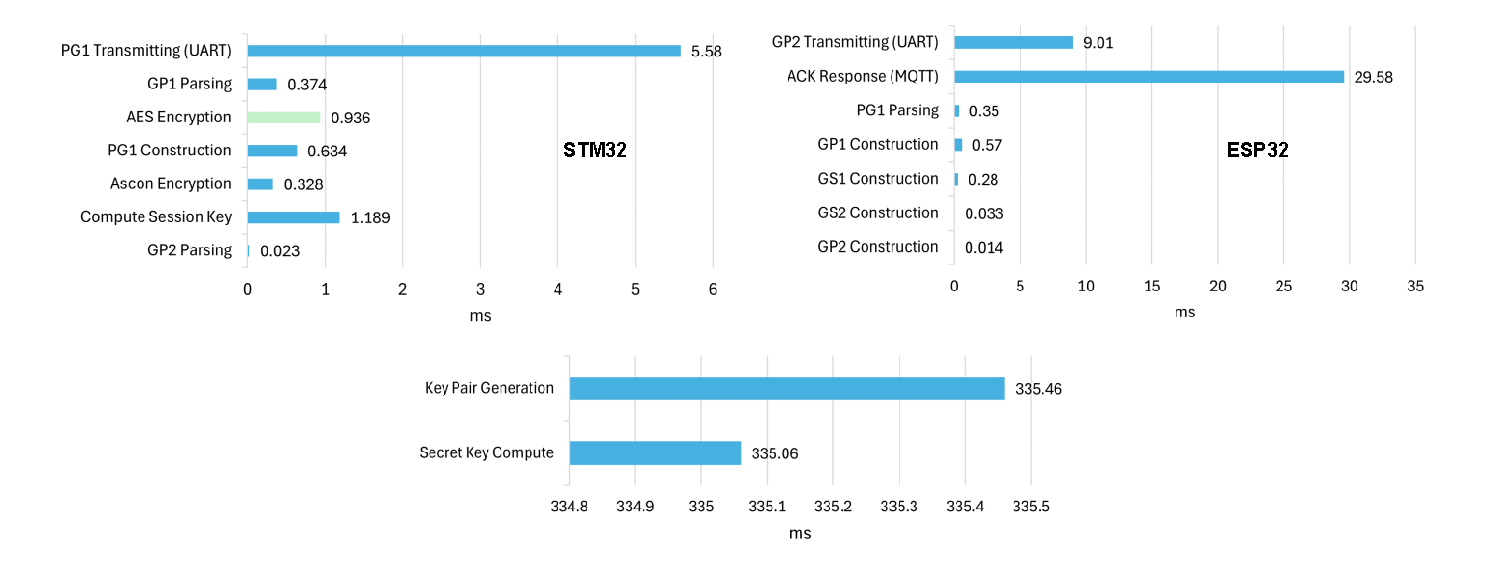
\includegraphics[width=1.2\textwidth]{pic/res_time.pdf}
	\end{figure}
\end{frame}

\begin{frame}{PACKET DELIVERY RATIO}
	\vspace{-0.25cm}
	\begin{figure}
		\centering
		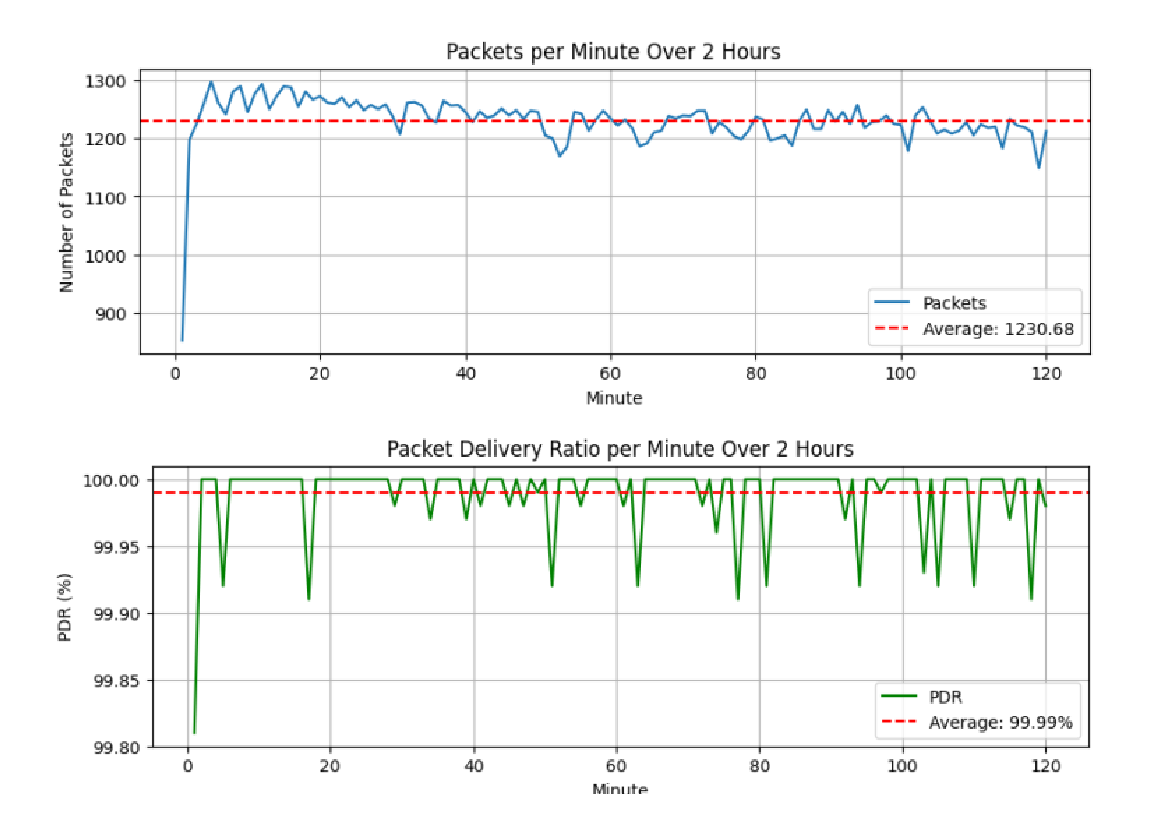
\includegraphics[width=0.65\textwidth]{pic/pdr.pdf}
	\end{figure}
\end{frame}

\begin{frame}{POWER CONSUMPTION}
	Công suất tiêu thụ trung bình là 779.43 mW.
	\vspace{-0.2cm}
	\begin{figure}
		\centering
		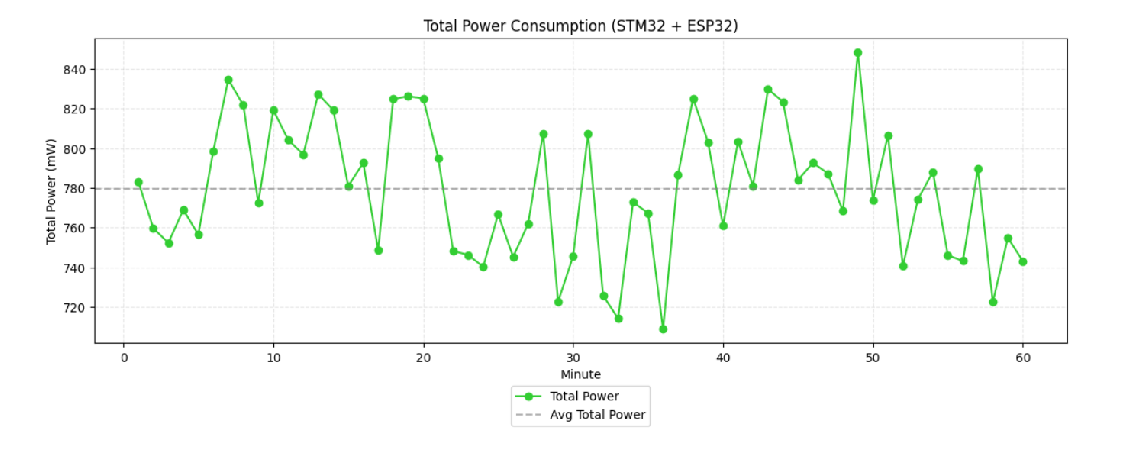
\includegraphics[width=1\textwidth]{pic/power.pdf}
	\end{figure}
\end{frame}

\begin{frame}{PAYLOAD EFFICIENCY}
	Đánh giá dựa trên khung truyền GS2 và kích thước dữ liệu là 3 bytes.
	\begin{figure}
		\centering
		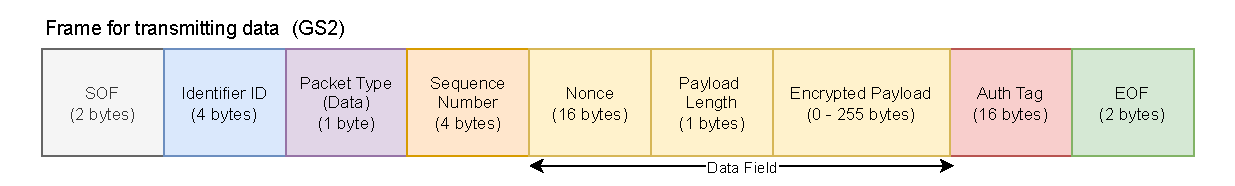
\includegraphics[width=1\textwidth]{pic/gs2.pdf}
	\end{figure}
	Với 3 bytes dữ liệu, tổng kích thước khung truyền là 49 bytes.
	$\Rightarrow \text{Hiệu suất tải dữ liệu là } \frac{3}{49} \approx 6.12\%$
\end{frame}

\begin{frame}{PAYLOAD EFFICIENCY}
	\begin{table}[h]
	\centering
	\small
	\caption{Hiệu suất tải với các kích thước tải khác nhau}
	\label{tab:efficiency}
	\begin{tabular}{|p{4cm}|p{5cm}|p{3cm}|}
	\hline
	Payload Length & Total Frame Size & Efficiency \\
	\hline
	3 bytes   & 49 bytes  & 6.12\%  \\
	10 bytes  & 56 bytes & 17.85\% \\
	20 bytes  & 66 bytes & 30.30\% \\
	50 bytes  & 96 bytes & 52.08\% \\
	\hline
	\end{tabular}
	\end{table}
	$\Rightarrow \text{Payload càng lớn thì hiệu suất tải dữ liệu càng cao}$
\end{frame}